TRITIUM-IFIC-0 was the first prototype developed in the TRITIUM project to check the feasibility of the technology proposed by TRITIUM, that is, to employ plastic scintillating fibers to detect tritium in water with good sensitivity. As liquid radioactive sources were involved, a special attention was paid to radiation safety in the design.

TRITIUM-IFIC-0 consists of a bundle of 35 fibers of $20~\cm$ length, which were cleaved and polished with the techniques reported in section \ref{sec:CharacterizationScintillatingFibers}. This bundle is attached to the vessel by means of metallic pieces located at its ends, as shown in Figure \ref{fig:FiberBundleOfTritiumIFIC0}. The PVC\footnote{Polyvinyl Chloride, PVC} vessel, shown in Figure \ref{fig:TritiumIFIC0}, was designed in a U-shape to improve radiological safety. However, this shape was not appropriate, as we learned afterwards. A frame of methacrylate and steel, shown in Figure \ref{fig:TritiumIFIC0}, was designed and built to hold the prototype. Two calibrated Hamamatsu R8520-06SEL PMTs \cite{DataSheetPMTs} were optically coupled to the fiber bundle by optical grease \cite{OpticalGrease}. The voltage divider circuit employed is shown in Figure  \ref{fig:VoltageDividerCircuit}. The high voltage was set to $-800~\volt$, at which the gains are $1.26 \cdot{} 10^6$ and $1.01 \cdot{} 10^6$, and the quantum efficiencies are $29.76\%$ and $28.66\%$ at $\lambda=430~\nano\meter$, respectively. The two PMTs were read out in coincidence by the electronics shown in Figure \ref{subfig:ElectronicConfiguraiton2PMT}.

\begin{figure}
\centering
    \begin{subfigure}[b]{0.5\textwidth}
    \centering
    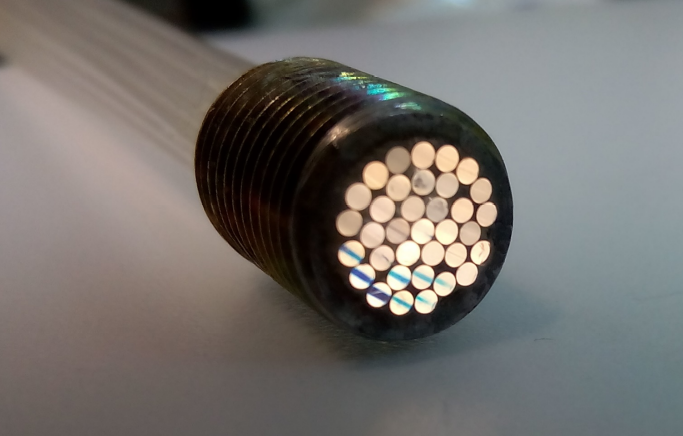
\includegraphics[width=\textwidth]{5Prototypes/52PreliminarPrototypes/521TritiumIFIC0/Metalic_piece_of_fiber_bundle.png}  
    \caption{\label{subfig:MetalicPieceFiberBunchTritiumIFIC0}}
    \end{subfigure}
    \hfill
    \begin{subfigure}[b]{0.4\textwidth}
    \centering
    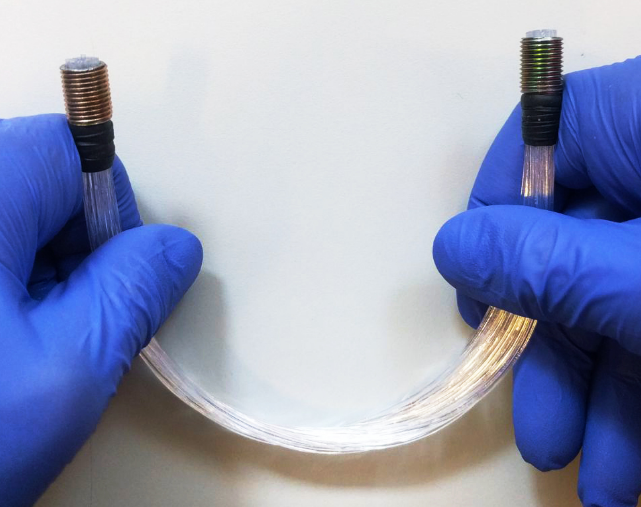
\includegraphics[width=\textwidth]{5Prototypes/52PreliminarPrototypes/521TritiumIFIC0/FiberBundleBent.png}  
    \caption{\label{subfig:FiberBunchTritiumIFIC0Bent}}
    \end{subfigure}
 \caption{a) Metallic piece of the fiber bundle. b) Bundle of $35$ fibers of $20~\cm$ length used in TRITIUM-IFIC-0.} \label{fig:FiberBundleOfTritiumIFIC0}
\end{figure}

\begin{figure}[h]
\centering
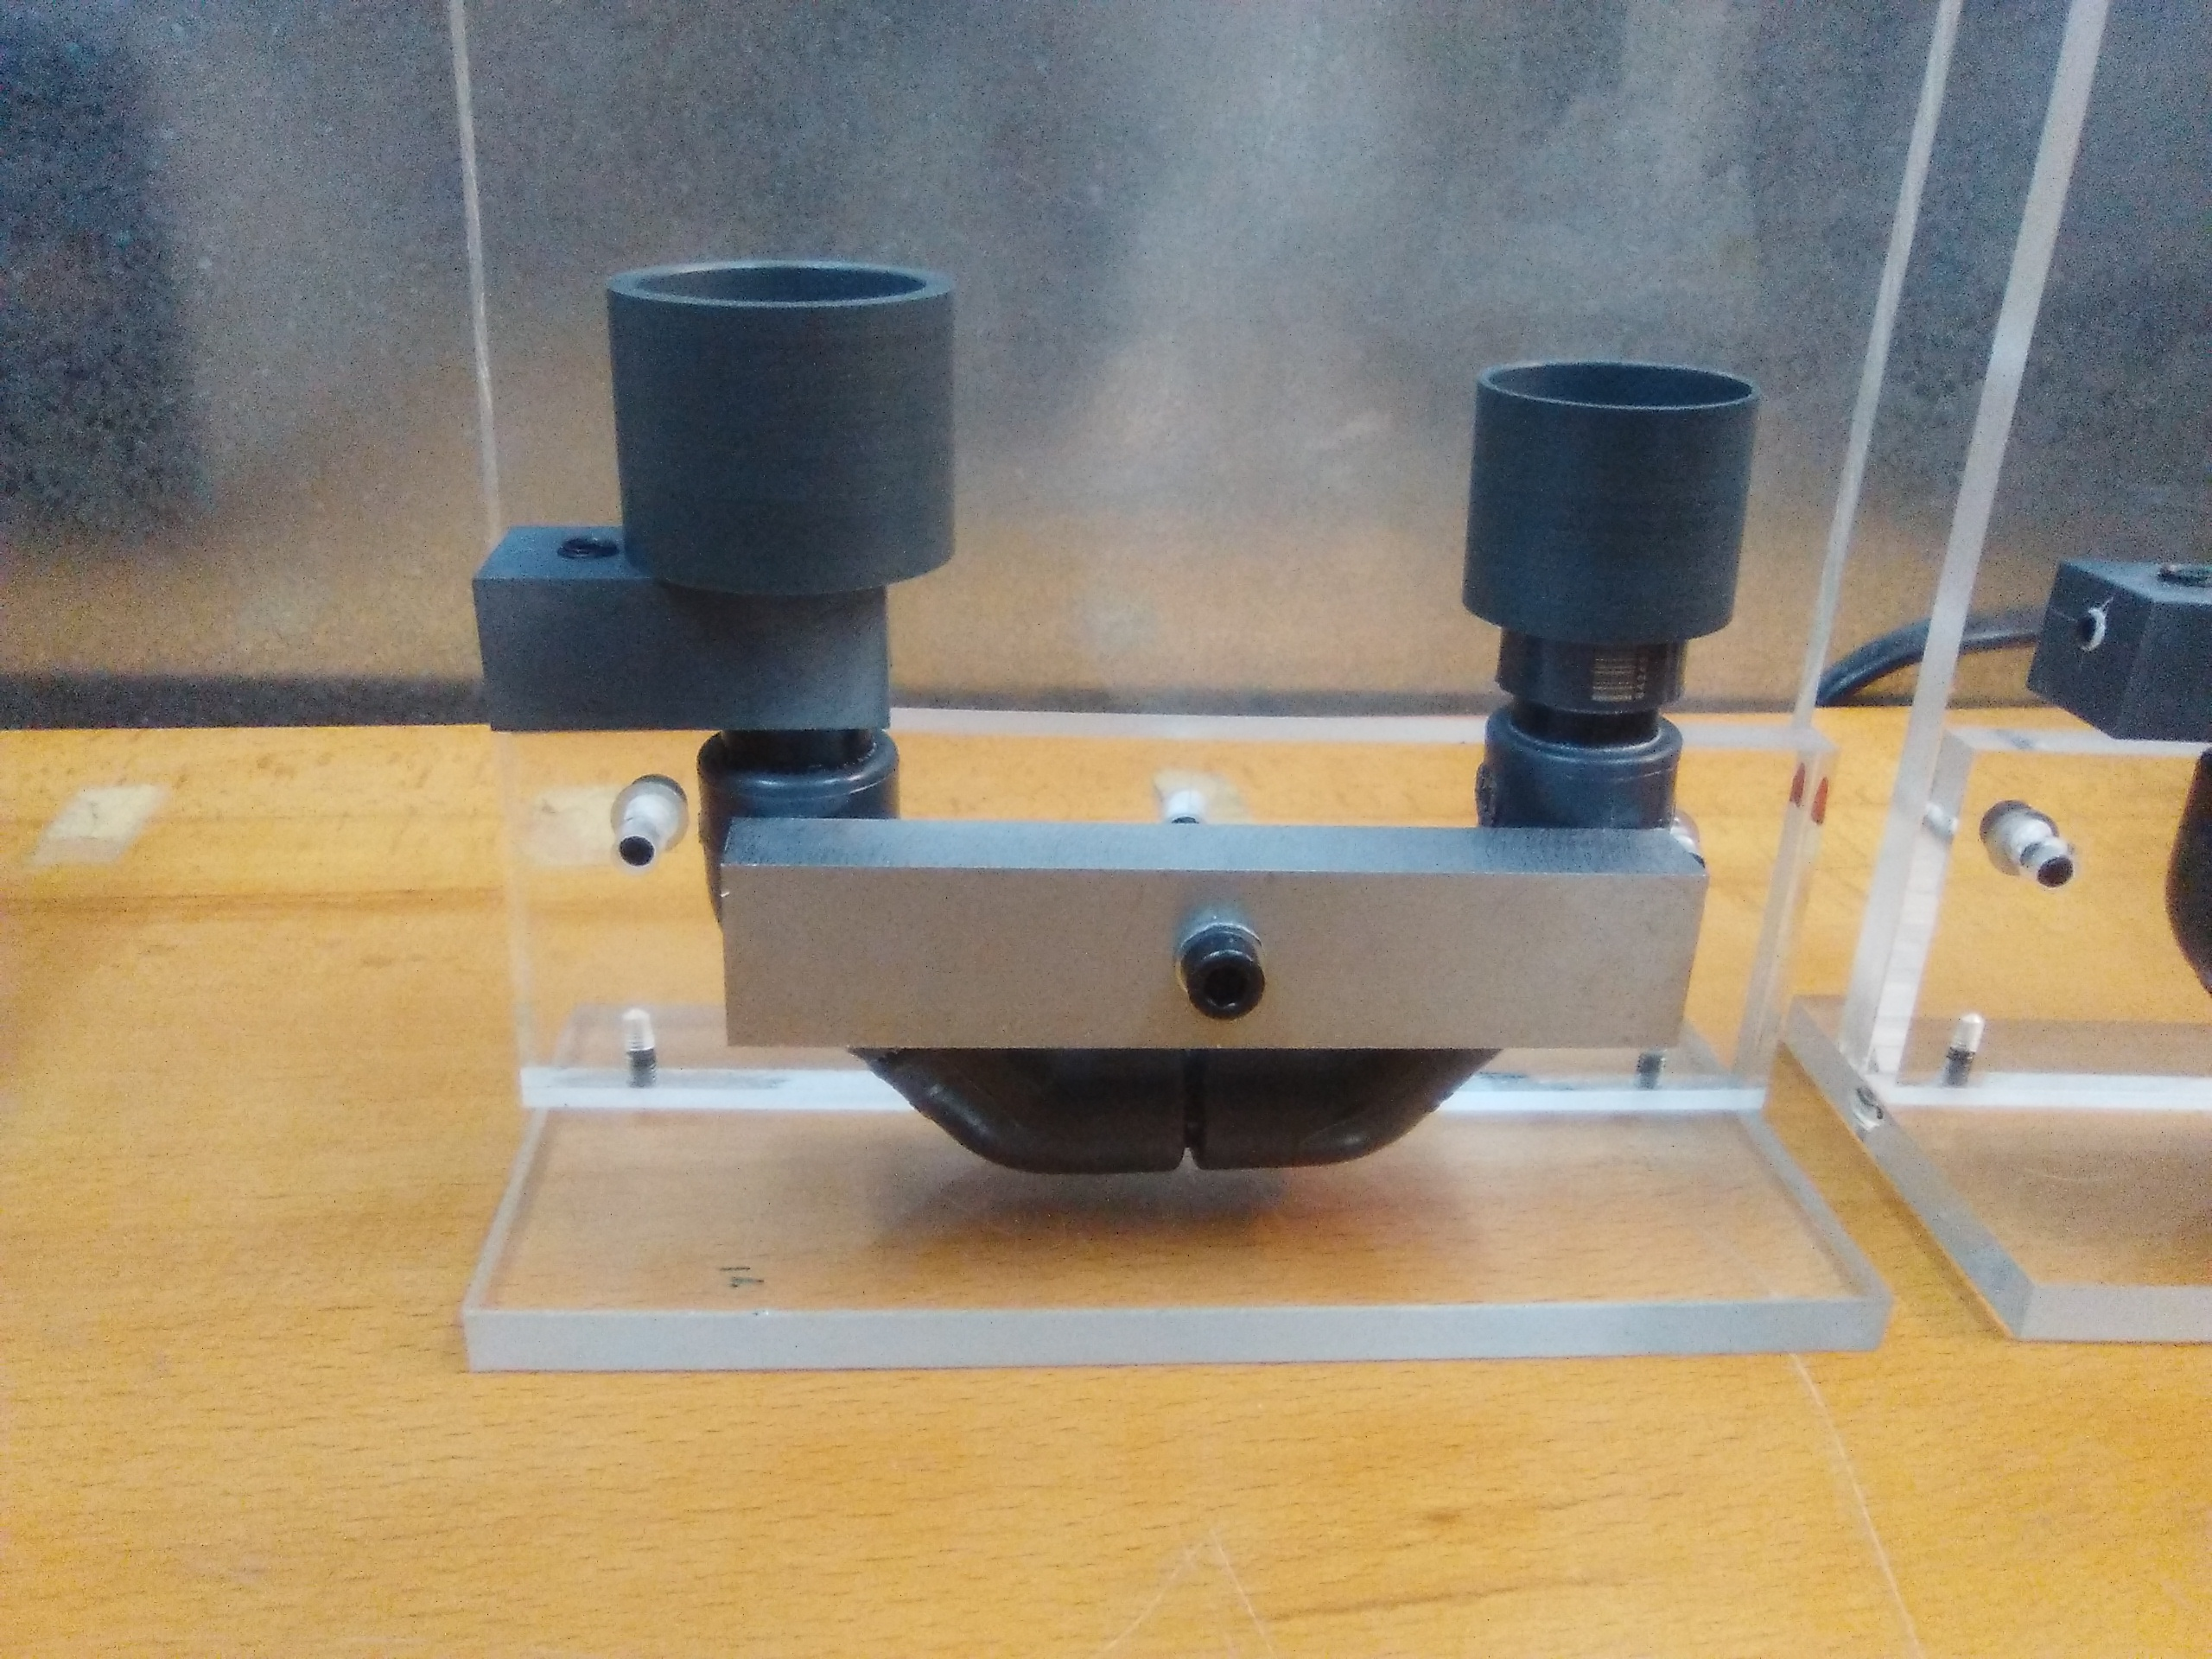
\includegraphics[scale=0.12]{5Prototypes/52PreliminarPrototypes/521TritiumIFIC0/Tritium_IFIC_0.jpg}
\caption{TRITIUM-IFIC-0 prototype.\label{fig:TritiumIFIC0}}
\end{figure}

Two identical prototypes were built. The first prototype, called ``TRITIUM-IFIC-0 Background'', was filled with pure water ($39~\milli\liter$, uncertainty of $0.05\%$) and was used to measure the background whereas the second prototype, called ``TRITIUM-IFIC-0 Signal'', was filled with a radioactive liquid source of tritiated water of a specific activity of $99.696~\kilo\becquerel/\liter$ (uncertainty of $2.24\%$) as reported in the appendix \ref{App:TritiumSourcePreparation}. This second prototype was employed to measure the total signal (tritium + background). The tritium signal was determined by substracting the background from the total signal. The number of time coincident events was too weak. The loss of photons was caused by several reasons, such as an excessive curvature of the fiber bundle due to the U-shape of the PVC vessel. Most of the photons escaped from the fibers due to both the shape of the bundle and the poor quality of the tritiated water-fiber interface (the implementation of the cleaning process described in section \ref{sec:CharacterizationScintillatingFibers} was motivated by this result). 

A transparent glass vessel similar to the TRITIUM-IFIC-0 prototype vessel, shown in Figure \ref{subfig:PMMAVesselToTestLostPhotons}, was built to study the effect of the fiber bundle curvature. The LED described in section \ref{sec:CharacterizationScintillatingFibers} was used to verify the reduction in photon collection efficiency of the fiber bundle due to its curvature. As can be seen in Figure \ref{subfig:TestLostPhotons}, most of the photons introduced from one side of the bundle do not reach the other side due to the fiber curvature. This test shows essential to keep a straight fiber arrangement in the design of the next prototypes. A second point is that the fiber bundle employed was too compact and water may not be able to flow around the fibers. In the TRITIUM-IFIC-1 prototype the fibers were sufficiently spaced by using a PTFE matrix.

\begin{figure}
\centering
    \begin{subfigure}[b]{0.45\textwidth}
    \centering
    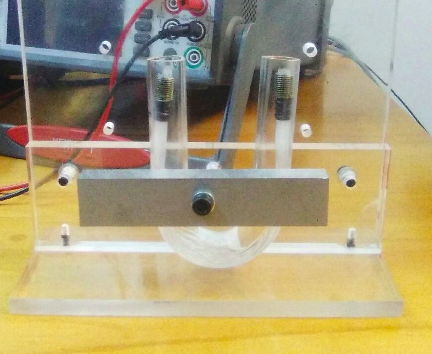
\includegraphics[width=\textwidth]{5Prototypes/52PreliminarPrototypes/521TritiumIFIC0/PMMA_vessel_ZOOM.png}  
    \caption{\label{subfig:PMMAVesselToTestLostPhotons}}
    \end{subfigure}
    \hfill
    \begin{subfigure}[b]{0.45\textwidth}
    \centering
    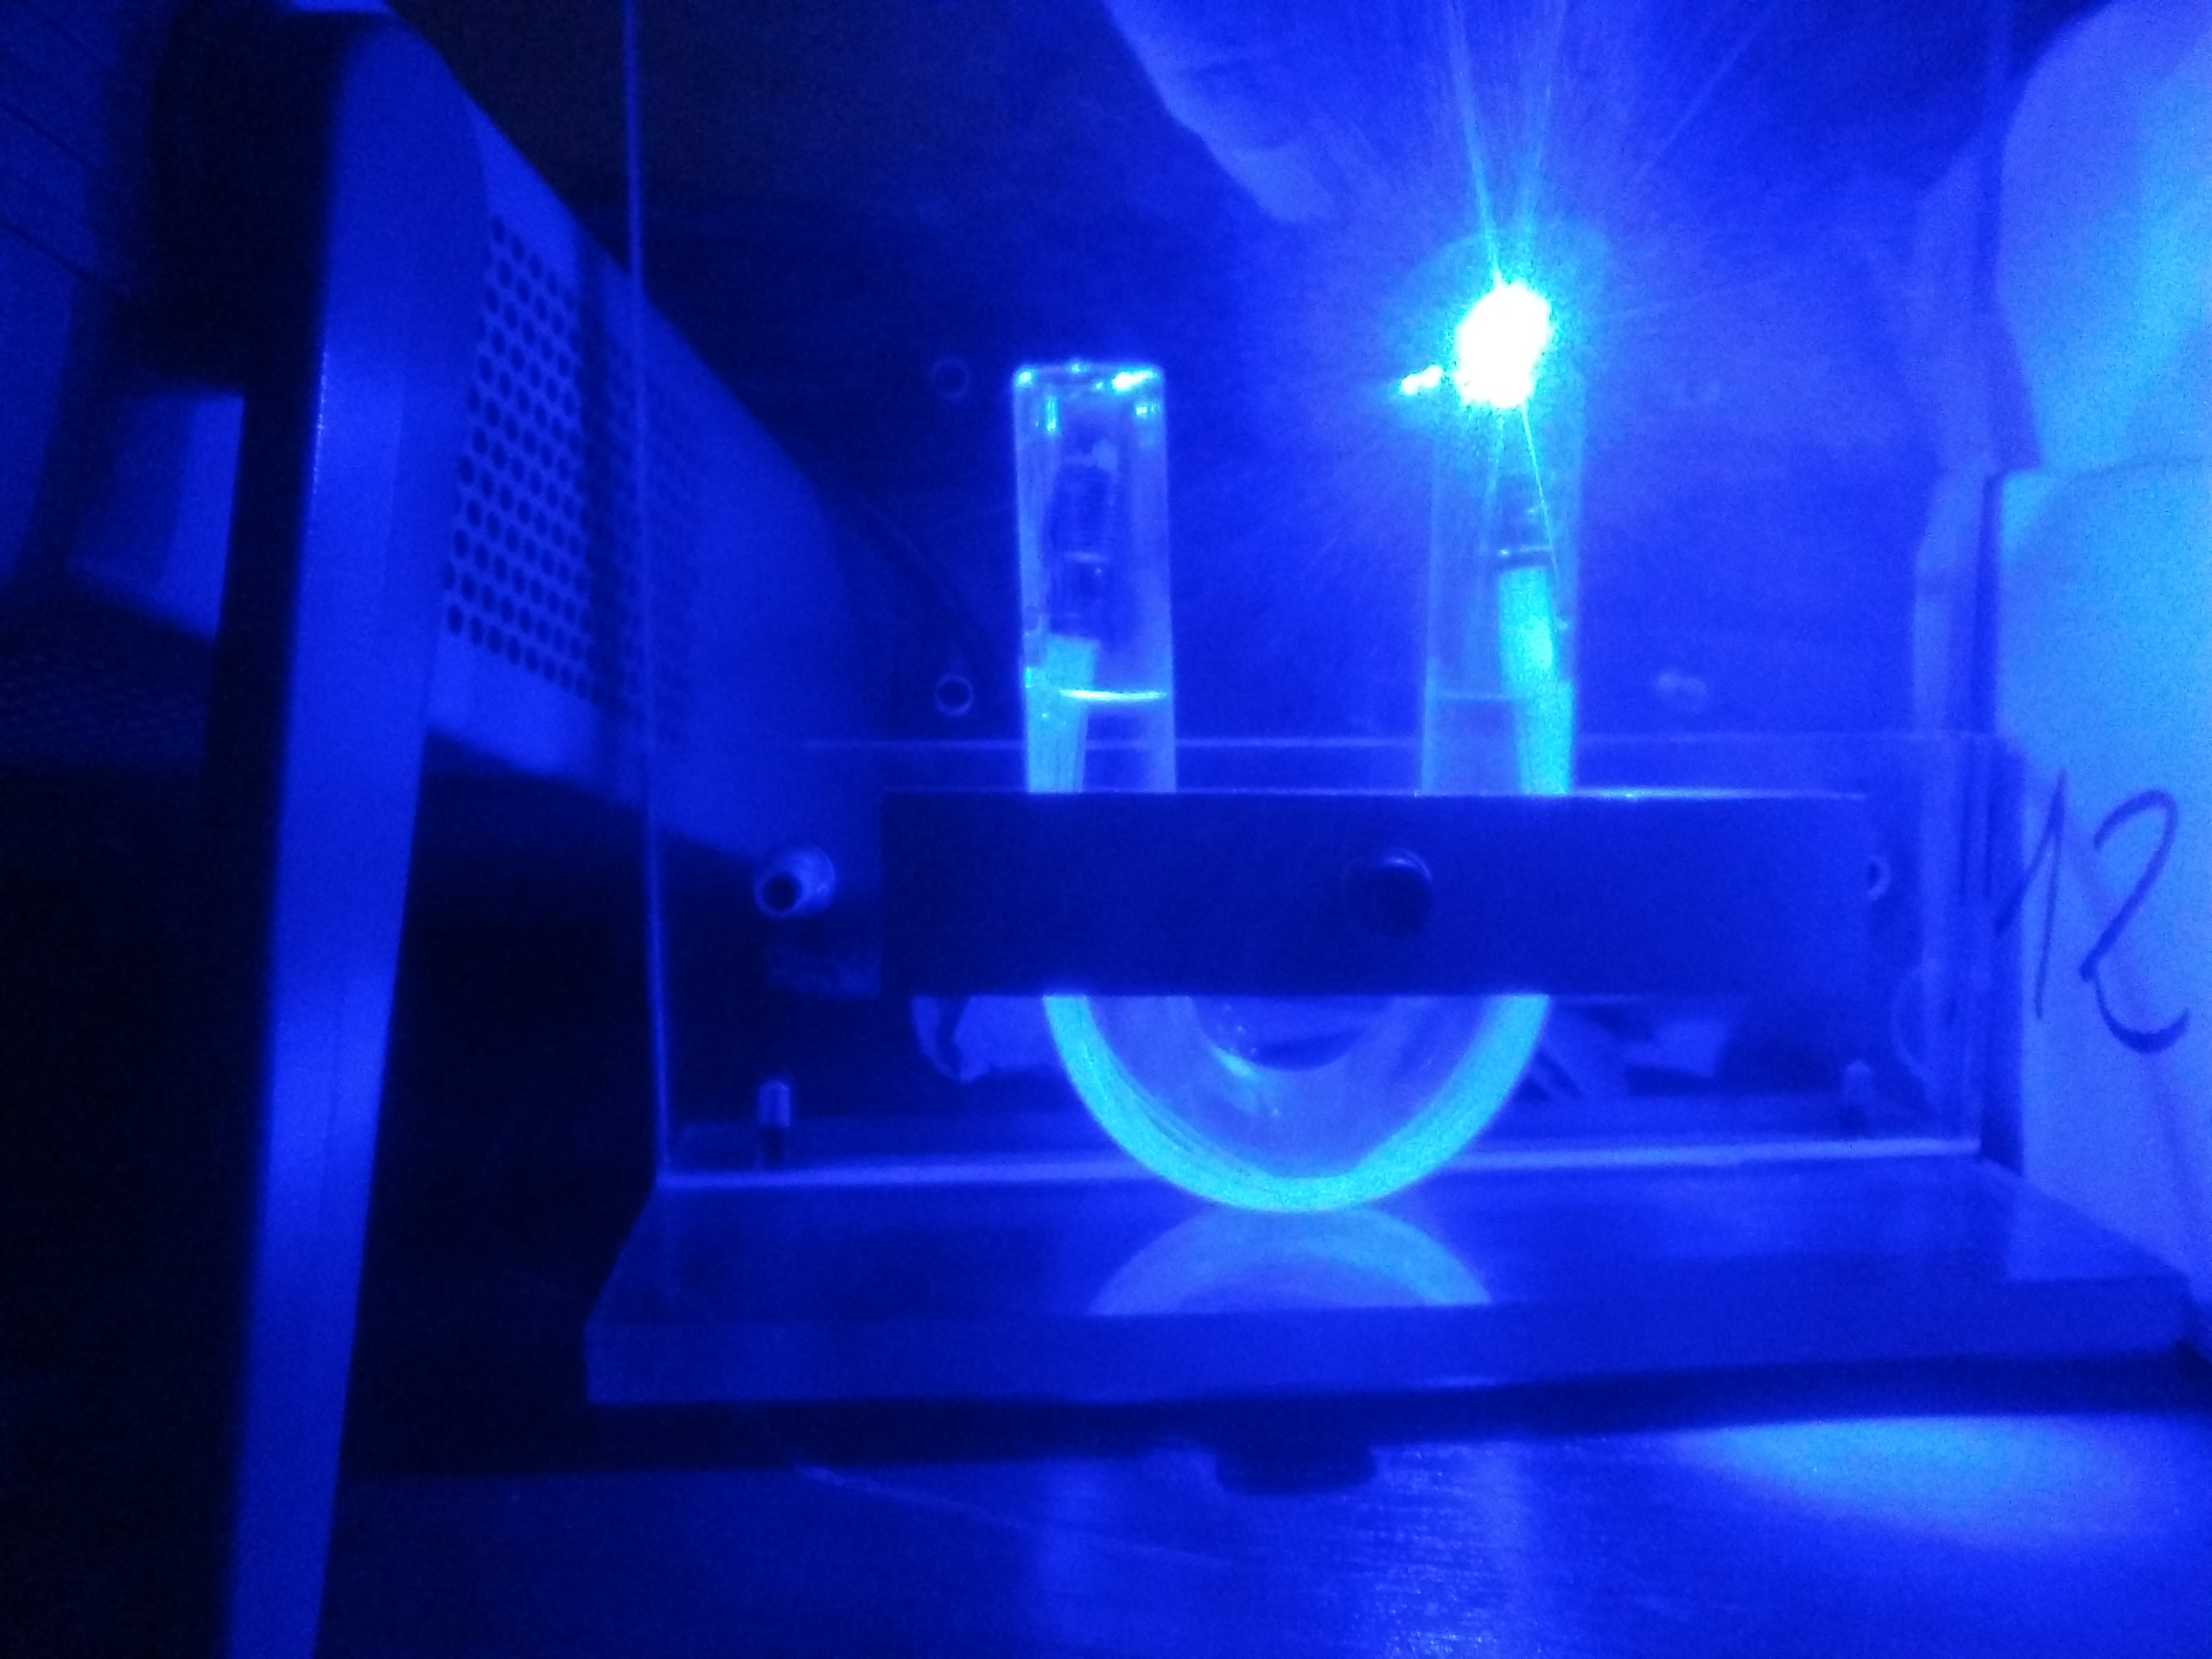
\includegraphics[width=\textwidth]{5Prototypes/52PreliminarPrototypes/521TritiumIFIC0/Lost_Photons.jpg}  
    \caption{\label{subfig:TestLostPhotons}}
    \end{subfigure}
 \caption{a) Fiber bundle in a PMMA vessel. b) Illumination test of the bundle to visualize the light loss due to fiber curvature.}
 \label{fig:TestLostPhotons}
\end{figure}

Data with TRITIUM-IFIC-0 were taken with a single PMT. The energy spectra measured for both the signal and background prototypes are shown in Figure \ref{subfig:SignalBackgroundEnergySpectraTritiumIFIC0}. The difference between signal and background, shown in Figure \ref{subfig:TritiumEnergySpectraTritiumIFIC0}, corresponds to the energy spectrum of tritium. The counting rate obtained for the three spectra are given in Table \ref{tab:CountsPerSecondTRITIUMIFIC0}.

\begin{figure}
\centering
    \begin{subfigure}[b]{1\textwidth}
    \centering
    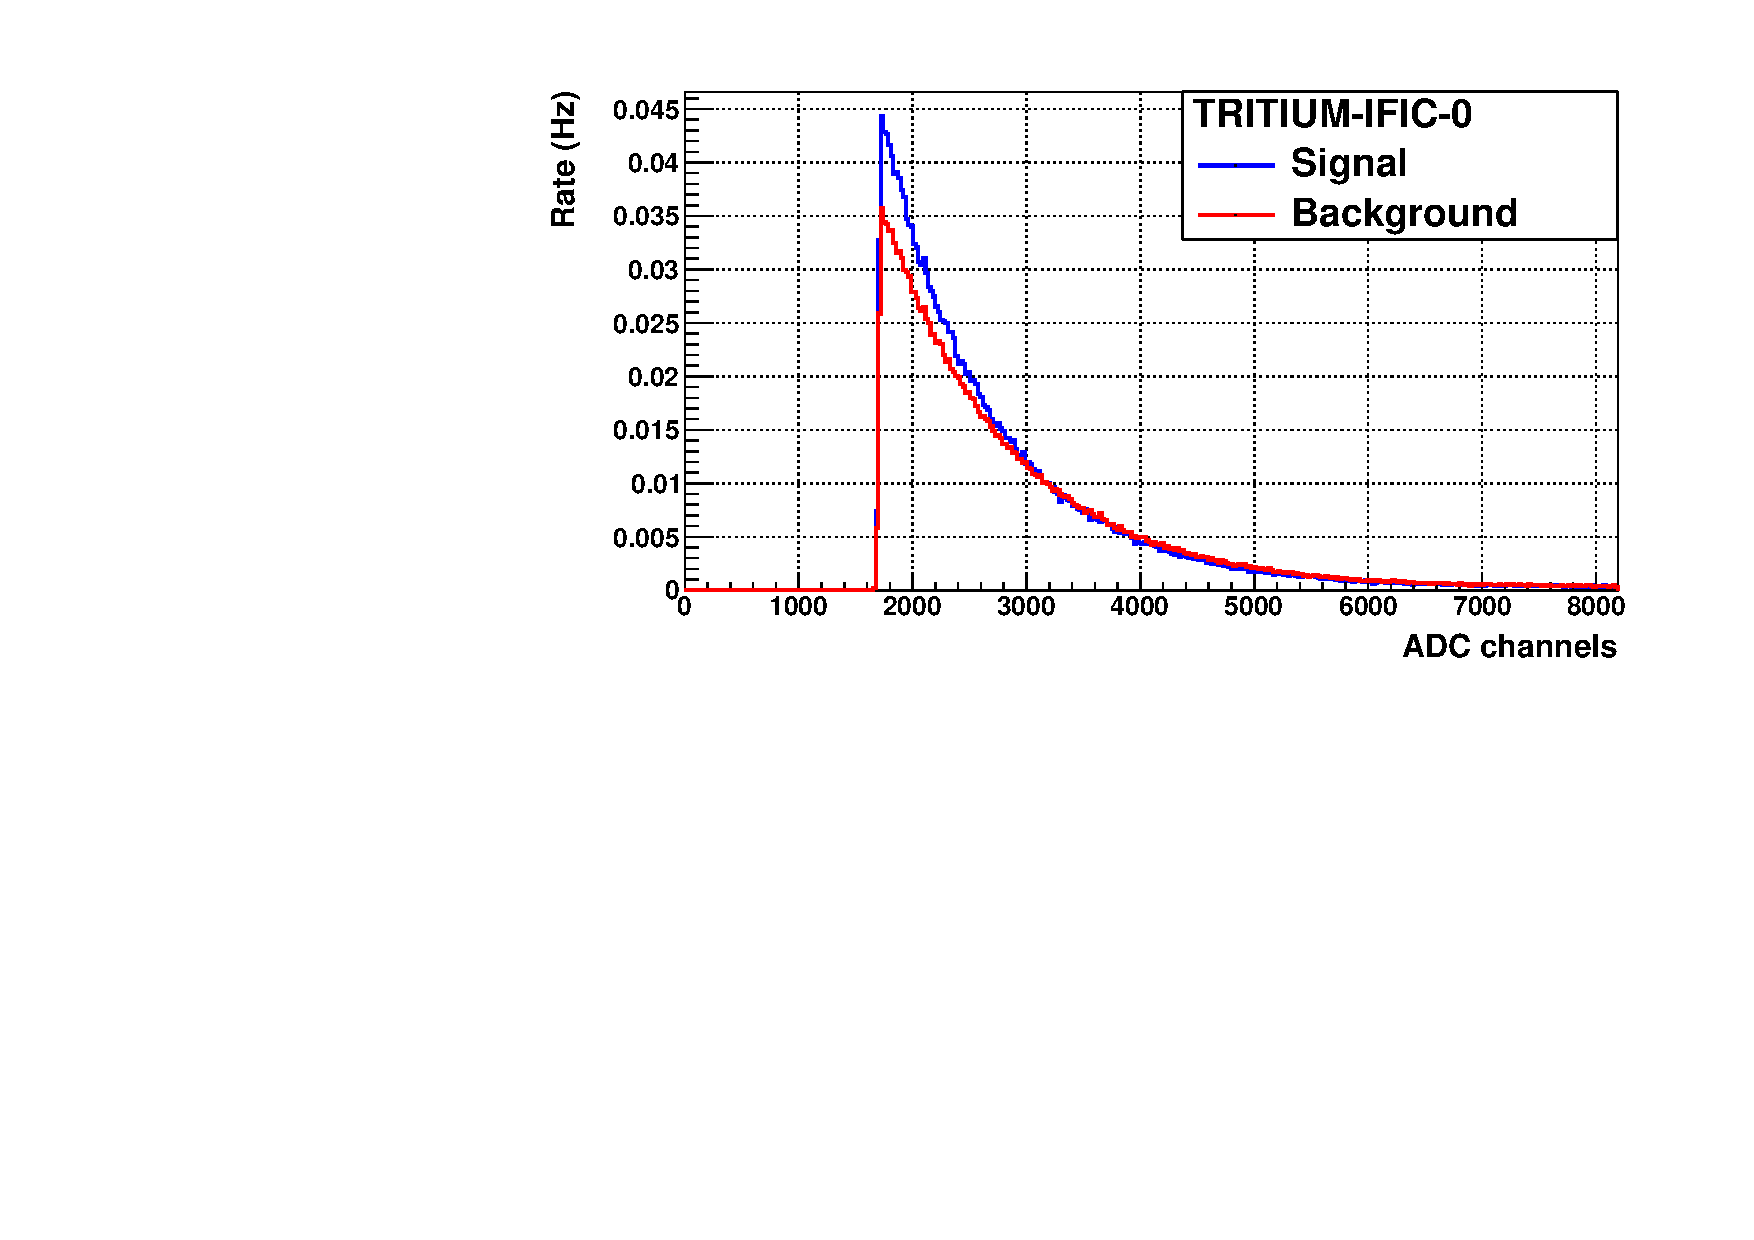
\includegraphics[width=\textwidth]{5Prototypes/52PreliminarPrototypes/521TritiumIFIC0/TritiumIFIC0Signals.pdf}  
    \caption{.\label{subfig:SignalBackgroundEnergySpectraTritiumIFIC0}}
    \end{subfigure}
    \hfill
    \begin{subfigure}[b]{1\textwidth}
    \centering
    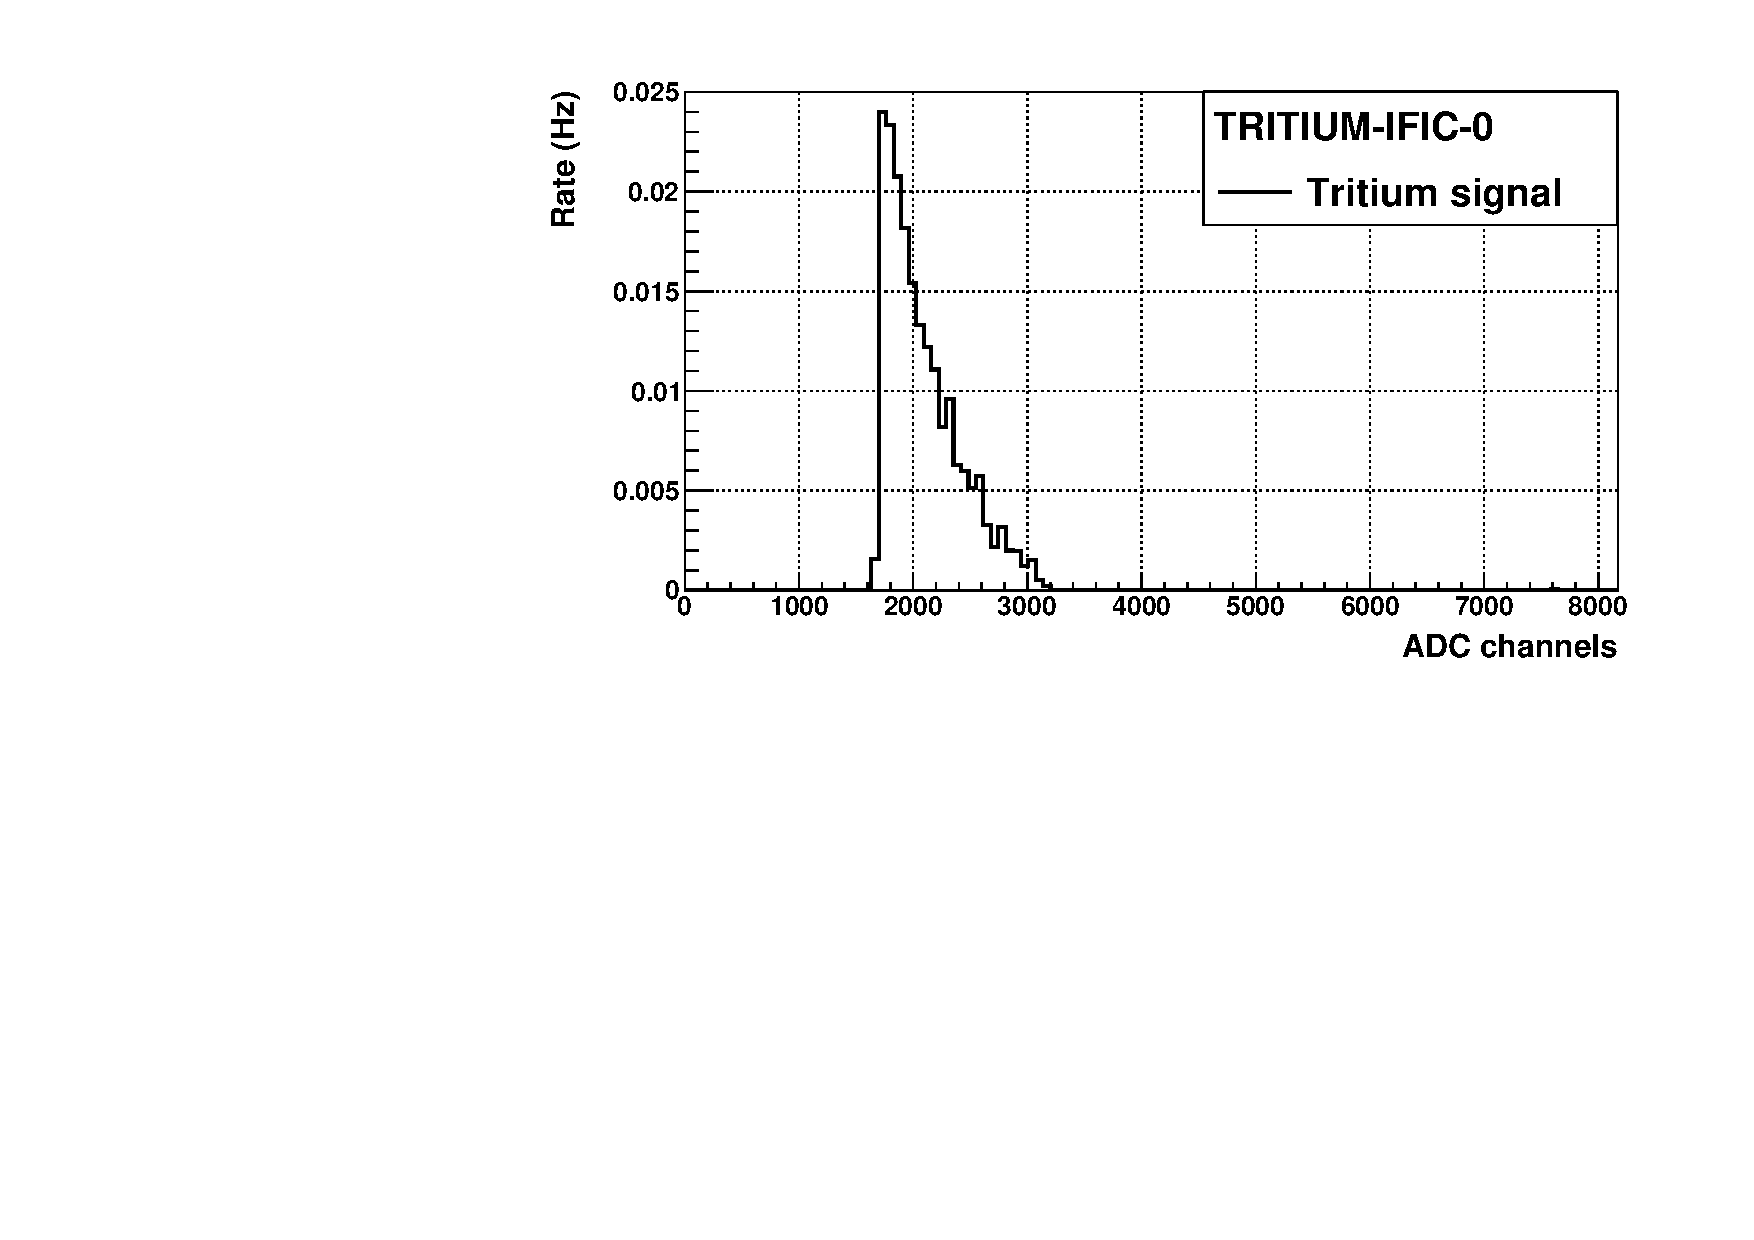
\includegraphics[width=\textwidth]{5Prototypes/52PreliminarPrototypes/521TritiumIFIC0/TritiumIFIC0ClearRebin.pdf}  
    \caption{\label{subfig:TritiumEnergySpectraTritiumIFIC0}}
    \end{subfigure}
 \caption{Energy spectra measured with TRITIUM-IFIC-0 prototype. a) Signal and background energy spectra. b) Tritium energy spectrum.}
 \label{fig:EnergySpectraTRITIUMIFIC0}
\end{figure}

\begin{table}[htbp]
\centering{}%
\begin{tabular}{cc}
\toprule 
Spectrum & Rate (Hz) \tabularnewline
\midrule
\midrule 
Signal & $2.27 \pm 0.06$ \tabularnewline
Background & $2.06 \pm 0.06$ \tabularnewline  
Tritium & $0.21 \pm 0.09$ \tabularnewline
\bottomrule
\end{tabular}
\caption{Rates obtained from the TRITIUM-IFIC-0 prototype.}
\label{tab:CountsPerSecondTRITIUMIFIC0}
\end{table}

The tritium detection efficiency obtained for this prototype is $$\eta=(2.1 \pm 0.9)\cdot{} 10^{-3}~\liter\:\kilo\becquerel^{-1}\second^{-1}$$, was calculated as the ratio of the tritium counting rate to the specific activity of the tritium liquid source. As reported in section \ref{sec:StateOfTheArt}, the tritium detection efficiency scales with the active area of the scintillator used. Therefore, to compare the efficiency with oher detectors in the literature and with other prototypes developed in the TRITIUM project, the specific efficiency $S$ of this prototype is calculated by normalizing to the scintillator area,
$$S = (9.6 \pm 3.9)\cdot{} 10^{-6}~\liter\:\kilo\becquerel^{-1}\second^{-1}\cm^{-2}$$
As can be seen in Table \ref{tab:PlasticScinTritium}, the specific efficiency is somewhat larger than that obtained by Muramatsu \cite{Muramatsu}, $S=3.13 \cdot{} 10^{-6}~\liter\:\kilo\becquerel^{-1}\second^{-1}\cm^{-2}$, and similar to that obtained by Moghissi \cite{Moghissi}, $S=10.6 \cdot{} 10^{-6}~\liter\:\kilo\becquerel^{-1}\second^{-1}\cm^{-2}$. These efficiencies are too low to achieve the objective of measuring activities of the order of $100~\becquerel/\liter$. 

%In addition, some improvements was applied to next prototype, Tritium-IFIC-1. On the one hand, the special cleaning protocol, previously explained in section \ref{subsubsec:CleaningProcess}, was applied on the fibers. It was used to improve the interfaces between fiber and tritiated water, creating a better wetting property of the fiber, which will result in more tritium events detected and a greater photon collection efficiency.

%On the other hand, as we have seen in our previous characterization study of the fibers, shown in section \ref{subsubsec:CharacterizationFibers}, the photon collection efficiency of the fibers used is poor, so a large number of photons will be lost in each tritium event.

%It is an innerent characteristic of the fiber which we cannot change but, to reduce its effect, we will use a Teflon vessel for our next prototypes.

%Teflon is an interesting material for its optical properties, specifically its reflection factor, which is very close to $100\%$ at the working wavelength. It means that practically all the photons that reach the walls of the vessel will be reflected back to the fiber.

%On the other hand, the fibers were inspected under the electronic microscope of the SCSIE \cite{ElectronicMicroscopeSCSIE}, with which we can see details of the order of tens of nanometers.

%The result is shown in Figure \ref{}, where you can see many irregularities of the order of $X~\nm$. These irregularities will cause photons to escape from the fiber. It is a characteristic of the fibers that we cannot change but, to reduce its effect, we will use a Teflon vessel for our next prototypes.

%FOTOOOO

%Teflon is an interesting material for its optical properties, specifically its reflection factor. Its reflection factor is very close to $100\%$ at the working wavelength, which means that practically all the photons that reach walls of the vessel will be reflected back to the fiber.